\documentclass{optica-article}

\journal{opticajournal}
\articletype{Research Article}

\usepackage{amsmath,mathtools,booktabs}
\usepackage{lineno}
\linenumbers % Comment out for arXiv or Optica Open preprint submission.
\emergencystretch=1.5em

\graphicspath{{figures/}}

\newcommand{\braket}[2]{\langle #1 | #2 \rangle}
\newcommand{\ket}[1]{\lvert #1 \rangle}
\newcommand{\bra}[1]{\langle #1 \rvert}
\newcommand{\norm}[1]{\lVert #1 \rVert}
\newcommand{\abs}[1]{\lvert #1 \rvert}
\newcommand{\dd}{\mathrm{d}}

\begin{document}

\title{Classical and quantum photonic protocols based on physical perfect optical vortex beam frames}

\author{Sebasti\'an Ayala\authormark{*}}

\address{Independent Researcher, Cauquenes, Chile\\
ORCID: \href{https://orcid.org/0009-0003-7348-3883}{0009-0003-7348-3883}}

\email{\authormark{*}ayala.phys.ds@gmail.com}

\begin{abstract*}
Physical perfect optical vortex beams (PVBs) form a continuous Hilbert frame whose azimuthal orbital angular momentum (OAM) sectors decouple orthogonally while radial overlap obeys a universal Gaussian kernel. We translate these frame primitives into four protocols across fiber, free-space, and quantum photonics: Sturm--Liouville coupling into step-index and parabolic graded-index ring-core fibers (reproducing the guided $l = 0\text{--}6$ window, $+6.97\,\mathrm{dB}$ launch gain, alignment tolerances, and multi-ring equalization); single-OAM discrete PVB dual-frame filtering in single- and five-screen Kolmogorov turbulence outperforming matched optimal Laguerre--Gaussian projectors; passive five-plane Gouy-diverse radial-qudit IC-POVM tomography across mixed, coherent, and Haar-random pure states; and circular-iris Bell--CHSH protection clearing the $82.84\%$ detection-loophole threshold at $1.048\,R_0$.
\end{abstract*}

\section{Introduction}
\label{sec:intro}

Structured optical wavefields carrying orbital angular momentum (OAM)~\cite{Allen1992,Erhard2018} enable high-capacity space-division multiplexing (SDM) in optical fibers and free space~\cite{Bozinovic2013,Willner2015} as well as high-dimensional quantum key distribution (QKD) and entanglement certification~\cite{Mirhosseini2015,Walborn2010}. In standard Laguerre--Gaussian ($\mathrm{LG}_{p,l}$) bases, however, the mode-dependent radial expansion $r_{\mathrm{rms}} = w_0\sqrt{2p+\abs{l}+1}$ induces asymmetric insertion loss in fixed-annulus ring-core fibers (RCFs)~\cite{Ramachandran2009,Zhang2018GRIN,RojasRojas2021,Canas2021,Asgharzadeh2026}, uneven modal crosstalk through atmospheric turbulence~\cite{Paterson2005,TylerBoyd2009,Roux2011,Ibrahim2013}, and $l$-dependent aperture side-channels in quantum receivers. Physical perfect optical vortex beams (PVBs)~\cite{Ostrovsky2013,Vaity2015,Reddy2016} confine all OAM orders to a common ring radius $R$ of finite half-width $w > 0$, supporting experimental telecom RCF transmission~\cite{Villalba2023} and recent second-order moment analyses~\cite{Ferreira2026}.

Harnessing physical PVBs beyond single-ring intensity carriers requires accounting rigorously for their radial nonorthogonality and continuous frame structure. In a companion theoretical study~\cite{AyalaV15Paper1}, it was established that finite-width PVBs form a continuous Bessel family on $L^2(\mathbb{R}^2)$ with isotropic Gaussian convolution frame operator $S_w = G_w * \cdot$ ($\widetilde{G}_w(k_\perp) = e^{-w^2 k_\perp^2/2}$), sharp Paley--Wiener stability bounds $A = e^{-w^2 k_{\max}^2/2}$ and $B = 1$ on bandlimited subspaces $\mathcal{H}_{k_{\max}}$, exact Fresnel propagation invariance $[S_w, \mathcal{U}_z] = 0$, an exact $(p+1)$-term closed-form expansion $c_{l,p}(R)$ for all $\mathrm{LG}_{p,l}$ modes ($p \ge 0$), and uniformly well-conditioned unit-normalized discrete radial Gram matrices $[\gamma]_{nm}$.

Here we develop and benchmark four classical and quantum photonic protocols enabled directly by these frame primitives. Section~\ref{sec:primitives} summarizes the necessary PVB frame relations and telecom $2f$ parameters. Section~\ref{sec:rcf_sdm} solves the Sturm--Liouville waveguide coupling problem for both step-index and parabolic graded-index (GRIN) RCFs, evaluates radial, width, and lateral alignment tolerances, and analyzes $N = 6$ concentric multi-ring SDM equalization~\cite{Fontaine2019,Fu2018,Berkhout2010,Proakis2008}. Section~\ref{sec:turbulence} evaluates single-OAM discrete PVB dual-frame filtering in both single-screen and five-screen split-step Kolmogorov turbulence~\cite{Lane1992,AndrewsPhillips2005}, benchmarking directly against an optimally waist-tuned matched-dimension $N = 5$ $\mathrm{LG}_{p,1}$ radial projector. Section~\ref{sec:povm} constructs passive multi-plane Gouy-diverse informationally complete POVM (IC-POVM) tomography~\cite{Gu2018,Zhou2017,Zhou2019,Choudhary2018,Renes2004,Lvovsky2004} of $d = 4$ radial photonic qudits across mixed, coherent, and Haar-random pure states under axial misalignment. Section~\ref{sec:chsh} analyzes circular-iris Bell--CHSH entanglement protection~\cite{Clauser1969,LawEberly2004,Walborn2010} and derives the pupil radius required to clear the $82.84\%$ symmetric detection-loophole threshold~\cite{Eberhard1993,Vertesi2010}. Section~\ref{sec:conclusions} concludes the paper.

\section{PVB Frame Primitives and Telecom Operating Point}
\label{sec:primitives}

Following Ref.~\cite{AyalaV15Paper1}, the continuous PVB frame elements at focal waist $z = 0$ are
\begin{equation}
  \Phi_{l,R}(r,\phi) = \frac{1}{w^2}\sqrt{\frac{2}{\pi}}\,e^{il\phi}\exp\!\left(-\frac{r^2+R^2}{w^2}\right) I_{\abs{l}}\!\left(\frac{2Rr}{w^2}\right),
  \label{eq:pvb_frame}
\end{equation}
whose resolution-of-identity prefactor fixes the optimal Bessel upper bound $B = 1$ under polar radial measure $\dd\mu(l,R) = R\,\dd R$. Physical single-channel overlaps and discrete Gram matrices use the unit-$L^2$-normalized states $\psi_{l,R} = \Phi_{l,R}/\norm{\Phi_{l,R}}_{L^2}$, where $\norm{\Phi_{l,R}}_{L^2}^2 = w^{-2} e^{-R^2/w^2} I_{\abs{l}}(R^2/w^2)$, yielding $[\gamma]_{nm} = \braket{\psi_{l,R_n}}{\psi_{l,R_m}} = I_{\abs{l}}(R_n R_m/w^2) / \allowbreak [I_{\abs{l}}(R_n^2/w^2) I_{\abs{l}}(R_m^2/w^2)]^{1/2}$.

For any unit-norm $\mathrm{LG}_{p,l}$ mode $\psi_{p,l}$ of waist $w_0$, the exact frame projection $c_{l,p}(R) = \braket{\Phi_{l,R}}{\psi_{p,l}}$ is given by the $(p+1)$-term closed form~\cite{AyalaV15Paper1}
\begin{equation}
  c_{l,p}(R) = \mathcal{A}_{p,l}(R)\sum_{m=0}^p (-1)^m \binom{p+\abs{l}}{p-m}\xi^m L_m^{\abs{l}}(-\zeta_R),
  \label{eq:c_lp}
\end{equation}
with $\xi = 2w^2/(w_0^2+w^2)$, $\zeta_R = R^2 w_0^2/[w^2(w_0^2+w^2)]$, and $\mathcal{A}_{p,l}(R) = 2^{\abs{l}/2+1}\sqrt{p!/(p+\abs{l})!}\,\allowbreak R^{\abs{l}} w_0^{\abs{l}+1}(w_0^2+w^2)^{-\abs{l}-1}\allowbreak\exp[-R^2/(w_0^2+w^2)]$. At telecom wavelength $\lambda = 1550\,\mathrm{nm}$ ($k_0 = 4.054\times 10^6\,\mathrm{m}^{-1}$), numerical aperture $\mathrm{NA} = 0.20$ ($k_{\max} = k_0\mathrm{NA} = 8.107\times 10^5\,\mathrm{m}^{-1}$), and RCF-matched half-width $w = 1.72\,\mu\mathrm{m}$, the space--bandwidth product is $w k_{\max} = 1.394$, yielding sharp Paley--Wiener frame bounds $A = \exp(-w^2 k_{\max}^2/2) = 0.378$, $B = 1$, and $\kappa(S_{w,k_{\max}}) = 2.64$.

\section{Step-Index and Graded-Index RCF Coupling, Launch Tolerances, and Multi-Ring SDM}
\label{sec:rcf_sdm}

\subsection{Step-Index versus Parabolic GRIN Sturm--Liouville Waveguide Coupling}

Under the weakly guiding scalar Helmholtz approximation ($\Delta n/n_{\mathrm{clad}} = 0.0229 \ll 1$), guided RCF eigenmodes $\psi_{\mathrm{RCF},l}(r,\phi) = (2\pi)^{-1/2} u_l(r) e^{il\phi}$ ($\int_0^\infty \abs{u_l}^2 r\,\dd r = 1$) satisfy the Liouville-symmetrized radial eigenvalue problem ($u_l(r) = \chi_l(r)/\sqrt{r}$)
\begin{equation}
  -\frac{\dd^2\chi_l}{\dd r^2} + \left[\frac{l^2 - \frac{1}{4}}{r^2} - k_0^2 n^2(r)\right]\chi_l(r) = -\beta_l^2\chi_l(r),
  \label{eq:rcf_ode}
\end{equation}
solved via symmetric tridiagonal finite differences ($N_r = 2500$ on $[0.01, 20.0]\,\mu\mathrm{m}$). To connect theory directly to telecom experiments using graded-index ring-core fibers~\cite{Zhang2018GRIN,Villalba2023}, we solve Eq.~\eqref{eq:rcf_ode} for both a step-index core ($n_{\mathrm{core}} = n_{\mathrm{clad}} + \Delta n$ on $r \in [r_1, r_2]$) and a parabolic GRIN ring profile
\begin{equation}
  n_{\mathrm{GRIN}}^2(r) = n_{\mathrm{clad}}^2 + \bigl(n_{\mathrm{core}}^2 - n_{\mathrm{clad}}^2\bigr)\max\!\left[0,\; 1 - \left(\frac{r - r_{\mathrm{mid}}}{a_{\mathrm{ring}}}\right)^2\right],
  \label{eq:grin_prof}
\end{equation}
sharing identical core geometry $r_1 = 6.0\,\mu\mathrm{m}$, $r_2 = 9.0\,\mu\mathrm{m}$ ($r_{\mathrm{mid}} = 7.5\,\mu\mathrm{m}$, $a_{\mathrm{ring}} = 1.5\,\mu\mathrm{m}$), $n_{\mathrm{clad}} = 1.444$, $\Delta n = 0.033$, and $\lambda = 1550\,\mathrm{nm}$.

\begin{table}[htbp]
  \centering
  \caption{Exact Sturm--Liouville Modal Coupling Efficiency $\eta_l$ for Step-Index and Guided Parabolic GRIN RCFs ($\lambda = 1550\,\mathrm{nm}$)}
  \label{tab:rcf_grin}
  \scriptsize
  \renewcommand{\arraystretch}{1.14}
  \begin{tabular}{@{}cccc@{\hspace{1.2em}}cccc@{}}
  \toprule
  & \multicolumn{3}{c}{\textbf{Step-Index RCF ($w = 1.72\,\mu$m)}} & \multicolumn{4}{c}{\textbf{Parabolic GRIN RCF ($w_{\mathrm{opt}} = 1.96\,\mu$m)}} \\
  \cmidrule(r){2-4}\cmidrule(l){5-8}
  $l$ & $n_{\mathrm{eff}}$ & $\eta_{\mathrm{PVB}}$ & $\Delta\eta_{\mathrm{fix}}$ (dB) & $n_{\mathrm{eff}}$ & $\eta_{\mathrm{PVB}}$ & $\eta_{\mathrm{LG}}$ ($3.22\,\mu$m) & $\Delta\eta_{\mathrm{fix}}$ (dB) \\
  \midrule
  0 & 1.46777 & 0.9931 & $+23.87$ & 1.46111 & 0.9931 & 0.0053 & $+22.73$ \\
  1 & 1.46738 & 0.9932 & $+17.12$ & 1.46072 & 0.9932 & 0.0217 & $+16.61$ \\
  2 & 1.46622 & 0.9934 & $+12.66$ & 1.45956 & 0.9932 & 0.0559 & $+12.50$ \\
  3 & 1.46430 & 0.9931 & $+9.38$ & 1.45764 & 0.9928 & 0.1142 & $+9.39$ \\
  4 & 1.46166 & 0.9916 & $+6.90$ & 1.45499 & 0.9918 & 0.1991 & $+6.97$ \\
  5 & 1.45831 & 0.9883 & $+4.99$ & 1.45163 & 0.9897 & 0.3076 & $+5.08$ \\
  6 & 1.45430 & 0.9825 & $+3.52$ & 1.44760 & 0.9856 & 0.4303 & $+3.60$ \\
  7 & 1.44966 & 0.9733 & $+2.39$ & \emph{cutoff} & --- & --- & --- \\
  8 & 1.44443 & 0.9587 & $+1.52$ & \emph{cutoff} & --- & --- & --- \\
  \bottomrule
  \end{tabular}
\end{table}

Table~\ref{tab:rcf_grin} and Fig.~\ref{fig:rcf_grin}(a) reveal two key physical results. First, because the parabolic GRIN ring carries $2/3$ of the integrated core index-volume of the step-index ring, it guides strictly $l = 0\text{--}6$ ($n_{\mathrm{eff}}(6) = 1.44760 > n_{\mathrm{clad}} = 1.444$, while $l \ge 7$ falls below cladding cutoff), explaining from first principles the $l = 1\text{--}6$ transmission manifold demonstrated by Villalba \emph{et al.}~\cite{Villalba2023}. Second, physical PVBs maintain uniform efficiency across every guided order: $98.52\%$ mean efficiency across $l = 0\text{--}8$ in the step-index RCF ($+6.90\,\mathrm{dB}$ gain over fixed-collimator $\mathrm{LG}_{0,4}$ at $w_0 = 3.22\,\mu\mathrm{m}$), and $99.11\%$ mean efficiency across the guided $l = 0\text{--}6$ manifold in the parabolic GRIN RCF ($w_{\mathrm{opt}} = 1.959\,\mu\mathrm{m}$, giving $+6.97\,\mathrm{dB}$ gain at $l = 4$, within $0.14\,\mathrm{dB}$ of the experimental $+6.83\,\mathrm{dB}$ benchmark~\cite{Villalba2023} and consistent with predictions in Ref.~\cite{RojasRojas2021}). Even channel-matched $\mathrm{LG}_{0,l}$ ($w_0 = 4.50\,\mu\mathrm{m}$) drops to $\eta_{\mathrm{LG}}(1) = 0.2039$ on low OAM orders.

\subsection{Launch Misalignment Tolerances and Multi-Ring SDM Equalization}

Practical fiber coupling demands robustness against ring-radius mismatch $\delta R$, half-width error $\delta w$, and transverse lateral decentering $\delta x$. Direct 1D and $256\times 256$ 2D overlap integration at $l = 4$ [Fig.~\ref{fig:rcf_grin}(b)] shows that GRIN-RCF coupling remains above $92.3\%$ for lateral decentering $\abs{\delta x} \le 0.50\,\mu\mathrm{m}$ ($97.4\%$ at $0.25\,\mu\mathrm{m}$), above $91.5\%$ for radial offset $\abs{\delta R} \le 0.50\,\mu\mathrm{m}$, and above $95.7\%$ across $\pm 30\%$ width mismatch ($\delta w/w \in [-0.30, +0.30]$), confirming generous experimental alignment tolerances.

In free-space or large-core multi-ring SDM links, $N$ concentric PVB channels spaced by $\Delta R \ge 2.0\,w$ can be demultiplexed using multi-plane light conversion (MPLC) or radial mode sorters~\cite{Fontaine2019,Fu2018,Berkhout2010} followed by $N\times N$ zero-forcing (ZF) equalization $\hat{\mathbf{s}} = \gamma^{-1}\mathbf{y}$~\cite{Willner2015,Proakis2008}. The per-channel SNR noise-enhancement penalties under correlated optical-amplifier noise ($\mathbb{E}[\boldsymbol{\varepsilon}\boldsymbol{\varepsilon}^\dagger] = \sigma^2\gamma$) and post-detection receiver AWGN ($\sigma^2\mathbb{I}_N$) are
\begin{equation}
  \mathcal{P}_{\mathrm{corr}} = \frac{1}{N}\operatorname{Tr}(\gamma^{-1}), \qquad \mathcal{P}_{\mathrm{AWGN}} = \frac{1}{N}\operatorname{Tr}(\gamma^{-2}).
  \label{eq:zf_penalties}
\end{equation}
For $N = 6$ rings at $\Delta R = 2.0\,w$ ($\kappa(\gamma) = 1.645$, $17.36\,\mathrm{dB}$ isolation~\cite{AyalaV15Paper1}), Eq.~\eqref{eq:zf_penalties} yields $\mathcal{P}_{\mathrm{corr}} = 1.032$ ($0.14\,\mathrm{dB}$) and $\mathcal{P}_{\mathrm{AWGN}} = 1.099$ ($0.41\,\mathrm{dB}$), yielding negligible on-off keying bit-error-rate penalty $\mathrm{BER} = \frac{1}{2}\operatorname{erfc}[\sqrt{\eta_l(E_b/N_0)/(2\mathcal{P})}]$ [Fig.~\ref{fig:rcf_grin}(a) inset].

\begin{figure}[htbp]
  \centering
  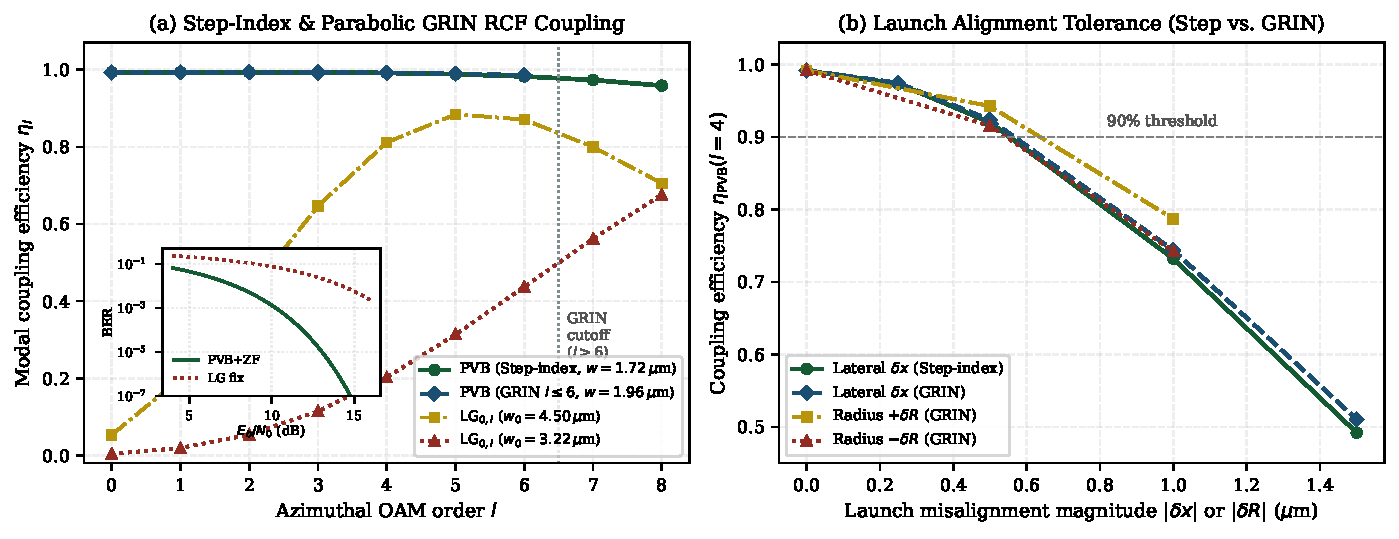
\includegraphics[width=0.98\textwidth]{fig1_rcf_step_grin_tolerances.pdf}
  \caption{RCF waveguide coupling, SDM BER, and launch alignment tolerances. (a) Exact Sturm--Liouville coupling $\eta_l$ across $l = 0\text{--}8$ for step-index and parabolic GRIN RCFs (marking the GRIN $l = 6$ cutoff) versus $\mathrm{LG}_{0,l}$; inset shows dispersion-free $l = 4$ OOK BER including the $0.41\,\mathrm{dB}$ ($N=6$) ZF equalization penalty. (b) Coupling tolerance at $l = 4$ versus lateral decentering $\delta x$ and ring-radius mismatch $\pm\delta R$.}
  \label{fig:rcf_grin}
\end{figure}

\section{Single-OAM Discrete PVB Dual-Frame Filtering in Atmospheric Turbulence}
\label{sec:turbulence}

Atmospheric Kolmogorov turbulence scatters OAM beams into high-$k_\perp$ radial speckles and neighboring azimuthal orders $l \neq l_0$~\cite{Paterson2005,TylerBoyd2009,Roux2011,Ibrahim2013,AndrewsPhillips2005}. Rotation-invariant Fourier filters---such as a circular pinhole $P_{k_{\max}}$ or isotropic Tikhonov filter---cannot reject non-axisymmetric $l \neq l_0$ crosstalk. Exploiting the azimuthal--radial decoupling of PVB frames, we project the received turbulent field $\psi_{\mathrm{turb}}$ orthogonally onto the propagated $N$-ring single-OAM subspace $\mathcal{V}_N = \operatorname{span}\{\psi_{l_0,R_n}^{(\mathrm{prop})}\}_{n=1}^N$ ($l_0 = 1$, $N = 5$ rings $R_n \in \{0.25, 0.625, 1.00, 1.375, 1.75\}\,\mathrm{mm}$, $\Delta R = 1.5\,w$, $\kappa(\gamma) = 3.70$) via the exact biorthogonal dual projector
\begin{equation}
  P_{\mathrm{PVB},l_0}\psi_{\mathrm{turb}} = \sum_{n,m=1}^{N} (\gamma^{-1})_{nm}\braket{\psi_{l_0,R_m}^{(\mathrm{prop})}}{\psi_{\mathrm{turb}}}\psi_{l_0,R_n}^{(\mathrm{prop})}.
  \label{eq:pvb_turb_proj}
\end{equation}
Because $\mathcal{U}_z$ is unitary, the propagated Gram matrix equals the waist Gram matrix identically, and every $l \neq l_0$ component lies strictly in $\ker(P_{\mathrm{PVB},l_0})$.

To establish an indisputably fair baseline against standard orthogonal modal receivers, we benchmark Eq.~\eqref{eq:pvb_turb_proj} not only against isotropic $P_{k_{\max}}$ and Tikhonov filters ($\alpha_{\mathrm{reg}} = e^{-(wk_{\max})^2} = 0.0183$), but also against a \emph{matched-dimension $N = 5$ single-OAM $\mathrm{LG}_{p,l_0}$ ($p = 0\text{--}4$) subspace projector} $P_{\mathrm{LG},l_0}$ whose waist is globally optimized ($w_0^{\mathrm{opt}} = 0.405\,\mathrm{mm}$) to capture $99.74\%$ of the clean propagated signal PVB energy ($R_0 = 1.0\,\mathrm{mm}$, $w = 0.25\,\mathrm{mm}$, $\lambda = 1550\,\mathrm{nm}$, $z = 0.5\,\mathrm{m}$, pupil $D_{\mathrm{ap}} = 3.0\,\mathrm{mm}$). We simulate 30 independent $256\times 256$ 3-octave subharmonic Kolmogorov phase screens~\cite{Lane1992} (piston, tip, and tilt removed) across $D/r_0 \in [0.5, 3.0]$, plus an extended 5-screen split-step volume turbulence cascade (20 trials, screen Fried parameter $r_{0,\mathrm{scr}} = r_{0,\mathrm{tot}}\,5^{3/5}$~\cite{Roux2011}).

\begin{table}[htbp]
  \centering
  \caption{Normalized Field MSE in Single-Screen (30 Trials) and 5-Screen Split-Step (20 Trials) Kolmogorov Turbulence}
  \label{tab:turbulence}
  \scriptsize
  \renewcommand{\arraystretch}{1.14}
  \begin{tabular}{@{}ccccccc@{\hspace{1.2em}}cccc@{}}
  \toprule
  \multicolumn{7}{c}{\textbf{(a) Single-Screen Kolmogorov Turbulence ($z = 0.5\,$m)}} & \multicolumn{4}{c}{\textbf{(b) 5-Screen Split-Step Volume}} \\
  \cmidrule(r){1-7}\cmidrule(l){8-11}
  $D/r_0$ & $P(l_0)$ & Raw & $P_{k_{\max}}$ & Tikhonov & Opt.\ $\mathrm{LG}_5$ & $\mathrm{PVB}_5$ & $D/r_0$ & Raw & Opt.\ $\mathrm{LG}_5$ & $\mathrm{PVB}_5$ \\
  \midrule
  0.5 & 0.965 & 0.0363 & 0.0893 & 0.0658 & 0.0043 & \textbf{0.0015} & 1.5 & 0.1953 & 0.0303 & \textbf{0.0254} \\
  1.0 & 0.913 & 0.0950 & 0.1353 & 0.1069 & 0.0105 & \textbf{0.0068} & 2.0 & 0.3577 & 0.0683 & \textbf{0.0574} \\
  1.5 & 0.803 & 0.2241 & 0.2415 & 0.2029 & 0.0284 & \textbf{0.0224} & 3.0 & 0.7178 & 0.1954 & \textbf{0.1878} \\
  2.0 & 0.742 & 0.2990 & 0.2956 & 0.2515 & 0.0418 & \textbf{0.0360} & & & & \\
  2.5 & 0.631 & 0.4594 & 0.4239 & 0.3690 & 0.0899 & \textbf{0.0829} & & & & \\
  3.0 & 0.572 & 0.5272 & 0.4689 & 0.4095 & 0.0988 & \textbf{0.0914} & & & & \\
  \bottomrule
  \end{tabular}
\end{table}

Table~\ref{tab:turbulence} and Fig.~\ref{fig:turbulence} show that $P_{\mathrm{PVB},1}$ outperforms every competitor across every turbulence strength. At $D/r_0 = 3.0$ (where raw $l_0 = 1$ azimuthal purity falls to $57.2\%$), single-screen field MSE drops $5.77\times$ from $0.5272$ to $0.0914$ (versus $0.4095$ for isotropic Tikhonov and $0.0988$ for optimally tuned $\mathrm{LG}_5$); at weak turbulence ($D/r_0 = 0.5$), PVB$_5$ achieves $2.97\times$ lower residual MSE than $\mathrm{LG}_5$ ($0.0015$ vs.\ $0.0043$) because the signal lies natively inside the PVB frame span without the $0.26\%$ truncation bias of a 5-mode Laguerre expansion. Under extended 5-screen split-step propagation, PVB$_5$ preserves a $3.82\times\text{--}7.70\times$ MSE reduction over raw fields and remains superior to optimal $\mathrm{LG}_5$ at every strength.

\begin{figure}[htbp]
  \centering
  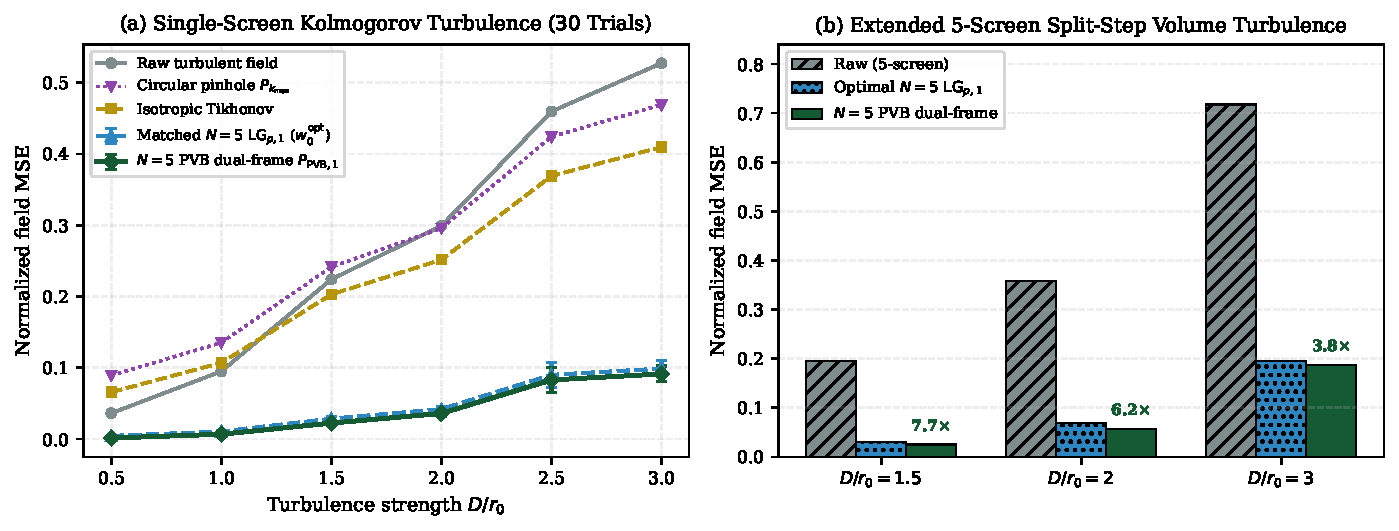
\includegraphics[width=0.98\textwidth]{fig2_turbulence_pvb_vs_lg.pdf}
  \caption{Kolmogorov turbulence spatial filtering. (a) Single-screen normalized field MSE ($\pm 1\,\mathrm{SEM}$, 30 trials) comparing raw distortion, $P_{k_{\max}}$, isotropic Tikhonov, optimally waist-tuned matched-dimension $N=5$ $\mathrm{LG}_{p,1}$ projector ($w_0^{\mathrm{opt}} = 0.405\,\mathrm{mm}$), and $N=5$ PVB dual-frame projector $P_{\mathrm{PVB},1}$. (b) Extended 5-screen split-step volume turbulence comparison (20 trials).}
  \label{fig:turbulence}
\end{figure}

\section{Passive Multi-Plane Gouy-Diverse Radial-Qudit IC-POVM Tomography}
\label{sec:povm}

Consider quantum state tomography on a $d$-dimensional fixed-$l$ radial photonic qudit space $\mathcal{H}_d^{(l)} = \operatorname{span}\{\ket{\psi_{p,l}}\}_{p=0}^{d-1}$~\cite{Gu2018,Zhou2017,Zhou2019,Choudhary2018}. At a single focal plane ($z = 0$), PVB intensity projections cannot be informationally complete (IC): because $c_{l,p}(R) \in \mathbb{R}$ in Eq.~\eqref{eq:c_lp}, every projector $\ket{\Phi_{l,R}}\bra{\Phi_{l,R}}$ vanishes on all $d(d-1)/2$ imaginary antisymmetric coherences; furthermore, since $c_{l,p}(R)$ factors into a $p$-independent envelope times a degree-$p$ polynomial in $\zeta_R$, all products $c_{l,p}(R)c_{l,p'}(R)$ span a polynomial space of dimension at most $2d - 1$. At $d = 4$, single-plane rank is strictly capped at $7/16 < 16$.

We lift this degeneracy passively without active modulator switching by splitting the photon across $M \ge d+1$ propagation planes $z_m$ sampling distinct Gouy phases $\vartheta_m = \arctan(z_m/z_R)$ ($z_R = k_0 w_0^2/2$). Employing the $\sigma_m^{+1}$-scaled wavefront-compensated PVB analyzers proven in Ref.~\cite{AyalaV15Paper1}, $\phi_{m,k}(r,\phi) = \sigma_m e^{+ik_0 r^2/[2R_c(z_m)]}\Phi_{l,\sigma_m R_k}(r,\phi;\,\sigma_m w)$ ($\sigma_m = \sqrt{1+(z_m/z_R)^2}$), defines the passive single-setting POVM elements~\cite{Renes2004}
\begin{equation}
  \Pi_{m,k} = \frac{R_k\Delta R}{M}\ket{\phi_{m,k}}\bra{\phi_{m,k}}, \qquad [\Pi_{m,k}]_{p,p'} = \frac{R_k\Delta R}{M} e^{-i 2(p-p')\vartheta_m} c_{l,p}(R_k) c_{l,p'}(R_k).
  \label{eq:ic_povm}
\end{equation}
Because the discrete bin sum approximates $(1/M)\sum_{m=1}^M P_{\mathcal{H}_d} S_w(z_m) P_{\mathcal{H}_d} \le \mathbb{I}_d$ by the Bessel upper bound $B = 1$, we obtain $\lambda_{\max}(\sum_{m,k}\Pi_{m,k}) = 0.9050 < 1$ for $d = 4$, $l = 1$, $w/w_0 = 0.25$, $M = 5$ planes ($\vartheta_m \in [0, 0.45\pi]$), and $K = 40$ midpoint bins on $(0, 3.5\,w_0]$, so the residual element $\Pi_{\mathrm{res}} = \mathbb{I}_d - \sum_{m,k}\Pi_{m,k} \ge 0$ completes the POVM rigorously.

In an orthonormal traceless Gell-Mann operator basis $\{B_j\}_{j=1}^{15}$, Eq.~\eqref{eq:ic_povm} lifts operator-frame rank from $7/16$ to full IC rank $16/16$ with $\kappa(\mathcal{S}_{\mathrm{POVM}}) = 442.5$ ($\kappa_{\mathrm{Bloch}} = 88.3$), classical Fisher condition number $\kappa(\mathbf{F}) = 14.86$, and single-photon Cram\'er--Rao bound at $\rho_0 = \mathbb{I}_4/4$:
\begin{equation}
  \operatorname{Tr}\!\left(\mathbf{F}^{-1}\right) = 41.80 \qquad \bigl(\text{vs.\ } \operatorname{Tr}(\mathbf{F}_{\mathrm{MUB}}^{-1}) = (d^2-1)(d+1)/d = 18.75\bigr),
  \label{eq:crb_povm}
\end{equation}
trading a modest $2.23\times$ photon-budget factor against sequential mutually unbiased bases (MUBs)~\cite{WoottersFields1989} for completely passive reconfiguration-free acquisition.

Going beyond maximally mixed states, we evaluate damped iterative $R\hat{\rho}R$ maximum-likelihood estimation (MLE)~\cite{Lvovsky2004} across: (1) the coherent radial superposition $\ket{\psi_{\mathrm{coh}}} = (\ket{0,1}+i\ket{3,1})/\sqrt{2}$ (25 trials per budget), (2) an ensemble of 20 Haar-random pure radial qudits at $N_{\mathrm{phot}} = 10^4$, and (3) uncalibrated axial plane positioning jitter $\delta z_{\mathrm{rms}}/z_R \in [0, 5\%]$ (Table~\ref{tab:povm_ext} and Fig.~\ref{fig:icpovm}). At $N_{\mathrm{phot}} = 10^4$, $\ket{\psi_{\mathrm{coh}}}$ reaches fidelity $F = 0.9823 \pm 0.0013$ (Frobenius MSE $1.54\times 10^{-3}$), the 20 Haar-random pure states achieve mean fidelity $0.9922$ (minimum $0.9833$), and even $5\%$ uncalibrated RMS axial positioning error degrades fidelity by only $0.006$ ($F = 0.9721$, perturbed $\mathrm{CRB} = 42.46$).

\begin{table}[htbp]
  \centering
  \caption{Passive $M=5$ Gouy IC-POVM Reconstruction of Coherent Superposition $\ket{\psi_{\mathrm{coh}}}$ and Axial-Jitter Robustness ($d=4, l=1$)}
  \label{tab:povm_ext}
  \scriptsize
  \renewcommand{\arraystretch}{1.14}
  \begin{tabular}{@{}ccc@{\hspace{1.8em}}ccc@{}}
  \toprule
  \multicolumn{3}{c}{\textbf{(a) Coherent State $\ket{\psi_{\mathrm{coh}}}$ Scaling (25 Trials)}} & \multicolumn{3}{c}{\textbf{(b) Uncalibrated Axial Jitter ($N_{\mathrm{phot}}=10^4$)}} \\
  \cmidrule(r){1-3}\cmidrule(l){4-6}
  $N_{\mathrm{phot}}$ & Fidelity $F(\hat{\rho},\psi_{\mathrm{coh}})$ & Frobenius MSE & $\delta z_{\mathrm{rms}}/z_R$ & Perturbed CRB & Fidelity $F$ \\
  \midrule
  $300$ & $0.9398 \pm 0.0082$ & 0.03658 & $0\%$ & 41.80 & 0.9779 \\
  $1{,}000$ & $0.9461 \pm 0.0057$ & 0.01827 & $1\%$ & 41.81 & 0.9826 \\
  $3{,}000$ & $0.9738 \pm 0.0028$ & 0.00581 & $3\%$ & 42.11 & 0.9766 \\
  $10{,}000$ & $0.9823 \pm 0.0013$ & 0.00154 & $5\%$ & 42.46 & 0.9721 \\
  $30{,}000$ & $0.9870 \pm 0.0008$ & 0.00067 & \multicolumn{3}{c}{\emph{20 Haar-random pure ($10^4$): $\bar{F}=0.9922$ (min $0.9833$)}} \\
  \bottomrule
  \end{tabular}
\end{table}

\begin{figure}[htbp]
  \centering
  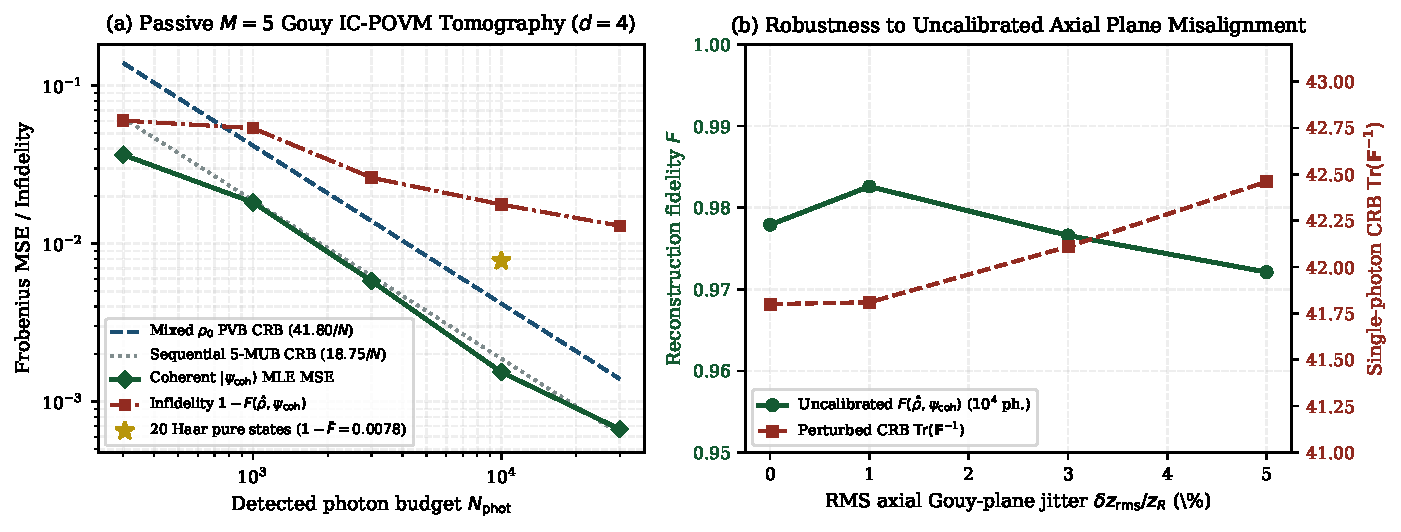
\includegraphics[width=0.98\textwidth]{fig3_gouy_icpovm_extended.pdf}
  \caption{Passive multi-plane Gouy IC-POVM tomography ($d=4, l=1, M=5, K=40$). (a) Frobenius MSE and infidelity $1-F$ for coherent superposition $\ket{\psi_{\mathrm{coh}}} = (\ket{0,1}+i\ket{3,1})/\sqrt{2}$ versus $N_{\mathrm{phot}}$ alongside PVB/5-MUB Cram\'er--Rao bounds and the 20-state Haar-random pure benchmark. (b) Uncalibrated reconstruction fidelity and perturbed CRB under axial Gouy-plane jitter $\delta z_{\mathrm{rms}}/z_R$.}
  \label{fig:icpovm}
\end{figure}

\section{Circular-Iris Bell--CHSH Preservation and Detection-Loophole Threshold}
\label{sec:chsh}

Behind a finite circular receiver aperture $\hat{T}_{\mathrm{iris}} = \Theta(R_{\mathrm{iris}} - r)$, standard $\mathrm{LG}_{0,l}$ modes suffer strongly $l$-dependent truncation governed by the regularized lower incomplete gamma function $t_l^{\mathrm{LG}}(R_{\mathrm{iris}}) = P(\abs{l}+1, 2R_{\mathrm{iris}}^2/w_0^2)$~\cite{LawEberly2004,Walborn2010}, introducing mode-dependent Procrustean entanglement decay and detection-efficiency side-channels.

By contrast, expanding unit-normalized PVB intensity around $r = R_0$ via Hankel's series ($w \ll R_0$) cancels both the polar radial Jacobian and the $\mathcal{O}((w/R_0)^2)$ constant term identically, pushing the leading $l$-dependent pupil transmission asymmetry to third order:
\begin{equation}
  t_l^{\mathrm{PVB}}(R_0) = \frac{1}{2} + c_0\frac{w}{R_0} - \frac{4l^2 - 1}{16\sqrt{2\pi}}\left(\frac{w}{R_0}\right)^3 + \mathcal{O}\!\left(\frac{w^5}{R_0^5}\right),
  \label{eq:t_pvb_asym}
\end{equation}
where $c_0$ is independent of $l$. For the two-photon OAM Bell state $\ket{\Psi} = (\ket{1,-1} + \ket{4,-4})/\sqrt{2}$~\cite{Clauser1969,Canas2021}, Horodecki optimization behind symmetric two-arm irises yields the post-selected Bell--CHSH parameter $S^{(2)} = 2\sqrt{1+\mathcal{V}^2}$ with $\mathcal{V} = 2t_1 t_4/(t_1^2 + t_4^2)$. Because $\delta_{14} \equiv (t_1 - t_4)/(t_1 + t_4) \approx [15/(4\sqrt{2\pi})](w/R_0)^3 = 1.496\times 10^{-3}$ at $w/R_0 = 0.1$, the deviation from Tsirelson's bound $2\sqrt{2}$ is suppressed to sixth order:
\begin{equation}
  0 < 2\sqrt{2} - S_{\mathrm{PVB}}^{(2)}(R_0) \approx 2\sqrt{2}\,\delta_{14}^2 = \mathcal{O}\!\left((l_1^2 - l_2^2)^2\left(\frac{w}{R_0}\right)^6\right),
  \label{eq:chsh_6th}
\end{equation}
giving $2\sqrt{2} - S_{\mathrm{PVB}}^{(2)}(R_0) = 6.48\times 10^{-6}$ ($1.62\times 10^{-6}$ one-arm) at $R_{\mathrm{iris}} = R_0$ (exact quadrature).

However, evaluating only $R_{\mathrm{iris}} = R_0$ clips $50\%$ of ring power ($24.9\%$ coincidence survival), preventing loophole-free Bell tests without fair sampling. To close the detection loophole on a maximally entangled two-qubit state with symmetric single-arm efficiency $\eta$, local hidden-variable bounds require $\eta > \eta_{\mathrm{crit}}^{\mathrm{CHSH}} = 2/(1+\sqrt{2}) = 82.8427\%$~\cite{Eberhard1993,Vertesi2010}. Sweeping $R_{\mathrm{iris}}/R_0$ and comparing fairly against three distinct $\mathrm{LG}_{0,l}$ waist calibrations---$l=4$ peak-matched ($w_0 = R_0/\sqrt{2}$), geometric-mean matched ($w_0 = R_0$), and $l=1$ peak-matched ($w_0 = \sqrt{2}R_0$)---demonstrates a dramatic aperture advantage for PVBs (Table~\ref{tab:chsh_loophole} and Fig.~\ref{fig:chsh_iris}): physical PVBs ($w/R_0 = 0.1$) clear $\min(t_1,t_4) \ge 82.84\%$ at $R_{\mathrm{iris}} = 1.0476\,R_0$, reach $95.5\%$ two-photon survival at $1.10\,R_0$, and attain $99.994\%$ two-photon survival with $2\sqrt{2} - S_{\mathrm{PVB}}^{(2)} = 1.28\times 10^{-13}$ at $1.20\,R_0$. Even the tightest $l=4$-matched LG baseline requires $R_{\mathrm{iris}} = 1.3243\,R_0$ ($1.60\times$ larger pupil area), while geometric-mean and $l=1$-matched LG modes require $1.8729\,R_0$ ($3.20\times$ area) and $2.6487\,R_0$ ($6.39\times$ area), respectively.

\begin{table}[htbp]
  \centering
  \caption{Circular-Iris Transmission, Two-Arm Bell--CHSH Parameter $S^{(2)}$, and Detection-Loophole Threshold$^a$ ($w/R_0 = 0.1$)}
  \label{tab:chsh_loophole}
  \scriptsize
  \renewcommand{\arraystretch}{1.14}
  \setlength{\tabcolsep}{4pt}
  \begin{tabular}{@{}ccccccc@{}}
  \toprule
  $R_{\mathrm{iris}}/R_0$ & $\min(t_1,t_4)_{\mathrm{PVB}}$ & $2\sqrt{2}-S_{\mathrm{PVB}}^{(2)}$ & Surv.$_{\mathrm{PVB}}^{(2)}$ & $S_{\mathrm{LG}}^{(2)}$ ($R_0/\sqrt{2}$) & $S_{\mathrm{LG}}^{(2)}$ ($R_0$) & $S_{\mathrm{LG}}^{(2)}$ ($\sqrt{2}R_0$) \\
  \midrule
  1.00 & 0.49841 & $6.48\times 10^{-6}$ & 0.2492 & 2.4416 & 2.0307 & 2.0008 \\
  1.10 & 0.97705 & $2.58\times 10^{-8}$ & 0.9548 & 2.6249 & 2.0754 & 2.0022 \\
  1.15 & 0.99864 & $1.52\times 10^{-10}$ & 0.9973 & 2.6924 & 2.1111 & 2.0036 \\
  1.20 & 0.99997 & $1.28\times 10^{-13}$ & 0.9999 & 2.7420 & 2.1570 & 2.0057 \\
  1.50 & 1.00000 & $<10^{-15}$ & 1.0000 & 2.8263 & 2.5593 & 2.0540 \\
  \bottomrule
  \end{tabular}

  \smallskip
  \noindent\parbox{0.96\textwidth}{\scriptsize $^a$Minimum iris radius clearing $\eta_{\mathrm{crit}}^{\mathrm{CHSH}} = 82.84\%$: PVB $= 1.0476\,R_0$; LG ($w_0=R_0/\sqrt{2}$) $= 1.3243\,R_0$ ($1.60\times$ pupil area); LG ($w_0=R_0$) $= 1.8729\,R_0$ ($3.20\times$ area); LG ($w_0=\sqrt{2}R_0$) $= 2.6487\,R_0$ ($6.39\times$ area).}
\end{table}

\begin{figure}[htbp]
  \centering
  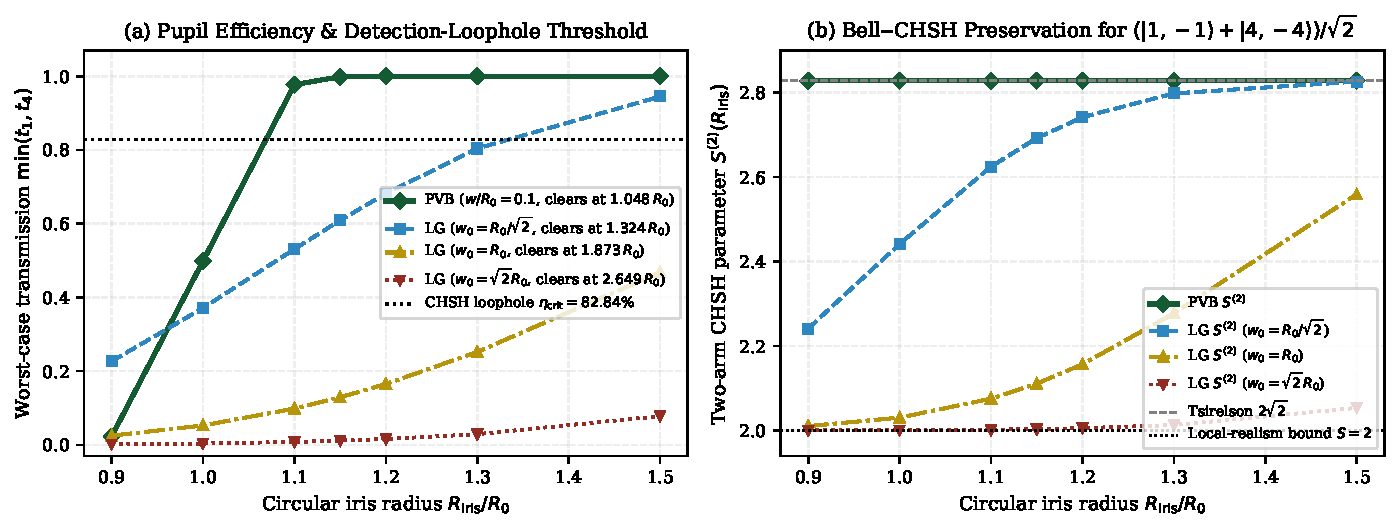
\includegraphics[width=0.98\textwidth]{fig4_iris_chsh_loophole.pdf}
  \caption{Circular-iris Bell--CHSH entanglement protection ($w/R_0 = 0.1$, $\ket{\Psi} = (\ket{1,-1}+\ket{4,-4})/\sqrt{2}$). (a) Worst-case single-photon transmission $\min(t_1,t_4)$ versus $R_{\mathrm{iris}}/R_0$ against three LG waist baselines and the $82.84\%$ symmetric CHSH detection-loophole threshold. (b) Two-arm post-selected CHSH parameter $S^{(2)}(R_{\mathrm{iris}})$ showing near-Tsirelson preservation across the full aperture range.}
  \label{fig:chsh_iris}
\end{figure}

\section{Conclusions}
\label{sec:conclusions}

Translating the continuous Hilbert frame theory of physical PVBs~\cite{AyalaV15Paper1} into concrete classical and quantum optical protocols demonstrates consistent operational advantages over conventional Laguerre--Gaussian architectures. First, exact Sturm--Liouville modeling of both step-index and parabolic GRIN ring-core fibers reproduces the guided $l = 0\text{--}6$ experimental manifold and $+6.97\,\mathrm{dB}$ PVB launch gain of Ref.~\cite{Villalba2023}, maintains $>91.5\%$ coupling across $\pm 0.5\,\mu\mathrm{m}$ radial/lateral misalignments, and incurs $\le 0.41\,\mathrm{dB}$ AWGN zero-forcing penalty across $N = 6$ concentric SDM channels. Second, single-OAM discrete PVB dual-frame filtering reduces Kolmogorov turbulence field MSE by up to $5.77\times$ ($3.82\times\text{--}7.70\times$ across five-screen volume propagation) and outperforms an optimally waist-tuned matched-dimension $N = 5$ $\mathrm{LG}_{p,1}$ projector at every turbulence strength. Third, passive five-plane Gouy-diverse PVB IC-POVM tomography reconstructs coherent radial superpositions and Haar-random pure qudits to fidelities $0.982\text{--}0.992$ at $10^4$ photons while tolerating $5\%$ uncalibrated axial plane jitter. Finally, circular-iris PVB transmission clears the $82.84\%$ symmetric Bell--CHSH detection-loophole threshold at $1.048\,R_0$, reducing required receiver pupil area by $1.60\times\text{--}6.39\times$ relative to Laguerre--Gaussian modes.

\begin{backmatter}
\bmsection{Funding}
This research received no external funding.

\bmsection{Acknowledgment}
The author acknowledges the use of standard symbolic and computational software tools for numerical verification and manuscript editing; all physical models, calculations, and interpretations are solely the responsibility of the author.

\bmsection{Disclosures}
The author declares no conflicts of interest.

\bmsection{Data availability}
Simulation scripts, benchmark datasets, and figure-generation code underlying the results presented in this paper are openly available in Ref.~\cite{AyalaCodeV15}.
\end{backmatter}

\bibliography{references}

\end{document}
